\addtocontents{toc}{\protect\newpage}

\chapter{Концептуальна модель формальної системи мов}
\epigraph{Присвячується автору ML, CCS, LCF та $\pi$-числення}{Артуру Джону Робіну Мілнеру}

Другий розділ описує розвиток концептуальної моделі системи доведення теорем як сукупності:
i) середовища виконання, яке складається з інтерпретатора та операційної системи;
ii) послідовності формальних мов програмування,
кожна наступна з яких, складніша за попередню,
має свою операційну семантику, та наслідує усі властивості
попередніх мов послідовності.

\section*{Вступне слово}
ML/LCF ---
LISP,LMI,CL/ACL2 ---
Smalltalk-80 ---
APL,K ---
BEAM ---

\section{Попередні відомості та теорії}
Для розповіді про систему доведення теорем, як систему мов програмування
будемо використовувати теорію категорії та теорію індуктивних
типів для специфікації синтаксисів мов програмування. Перелік необхідних формальних теорій:
лямбда числення, теорії індуктивних типів, вищі рівності для гомотопічної системи
тощо, містяться в розділі 3. Формальна теорія категорії міститься у розділі 4.
Слід зауважити, що ця формалізація проводиться на основі гомотопічної
мови програмування побудованої в даному розділі 2.

\begin{definition} (Концепт, Готлоб Фреге).
Концепт --- це предикат над об'єктом,
або іншими словами залежний $\Pi$-тип з теорії типів Мартіна-Льофа.
Об'єкт $x : o$ належить до концепту, тільки якщо сам концепт,
параметризований цим об'єктом, населений $p(o) : U$, де $p : concept(o)$.
\end{definition}

\begin{definition} (Система).
Визначимо систему як сукупність об'єктів $Ob : U$
та зв'язків між ними $Hom : Ob \rightarrow Ob \rightarrow U$.
\end{definition}

\begin{definition} (Концептуальна модель).
Таким чином концептуальна модель визначається як категорія, об'єкти якої
індексовані певною множиною, або залежні від параметра.
\end{definition}

\begin{definition} (Синтаксичне дерево).
Синтаксичне дерево --- це індуктивний тип або дерево Бома,
контруктори якого відповідають одному з 5 правил в теорії типів,
як правило використовуються три правила: правило формації, інтро-правила та елімінатор.
\end{definition}

\begin{definition} (Вище синтаксичне дерево).
Синтаксичне дерево в яке додано $\beta$ та $\eta$ правила називається
вищим синтаксичним деревом.
\end{definition}

\begin{definition} (Мова програмування).
Мова програмування або мовна категорія --- це категорія,
об’єкти якої --- це maybe-типи сум синтаксичних дерев мов програмування,
  а морфізми --- це стрілки (які містять правила виводу, типизації, нормалізації, екстакції тощо).
Приклади синтаксичних дерев: $O_\Pi$, $O_\Sigma$, $O_=$.
Приклади мовних категорій: $O_{PTS}$, $O_{MLTT}$, $O_{HTS}$.
\end{definition}

\begin{definition} (Модель).
Модель визначимо як систему формальних мов (об'єкти) разом з їх програмами,
та мовними перетвореннями (звязки) між ними для яких працює правило асоціативності
композиції та правила лівої і правої композиції з одиничними стрілками.
Іншими словами будемо розуміти тут категорну модель.
\end{definition}

\begin{definition} (Послідовність синтаксичних дерев). Кожна послідовність
синтаксичних дерев
\begin{equation}
O_\Pi \rightarrow O_\Sigma \rightarrow O_= \rightarrow O_W \rightarrow O_I.
\end{equation}
генерує відповідну послідовність мов програмування
\begin{equation}
\begin{split}
O_{PTS}(O_\Pi) \rightarrow O_{CTX}(O_\Pi,O_\Sigma) \rightarrow O_{EQU}(..,O_\Sigma,O_=) \rightarrow \\
 \quad \rightarrow O_{ITS}(...,O_=,O_W) \rightarrow O_{HTS}(...,O_W,O_I).
\end{split}
\end{equation}
наступним чином. Кожна мова програмування залежить
від синтаксису який її визначає
та всіх попредніх синтаксисів мов програмування з послідовності.
Перша мова програмування містить тільки перший синтаксис.
Розкриті сигнатури мають вигляд:
$O_{PTS}: O_\Pi \rightarrow U$,
$O_{CTX}: O_\Pi \rightarrow O_\Sigma \rightarrow U$,
$O_{EQU}: O_\Pi \rightarrow O_\Sigma \rightarrow O_= \rightarrow U$,
$O_{ITS}: O_\Pi \rightarrow O_\Sigma \rightarrow O_= \rightarrow O_W \rightarrow U$,
$O_{HTS}: O_\Pi \rightarrow O_\Sigma \rightarrow O_= \rightarrow O_W \rightarrow O_I \rightarrow U$.
\end{definition}

Таким чином кожна наступна мова програмування містить усі попередні
мови програмування, визначені послідовністю синтаксичних дерев,

\begin{definition} (Створення мовної категорії).
Мови можна додавати, наприклад $O_{HTS} = O_{\Pi\Sigma=WI}$, для побудови якої необхідно
об'єднати у індуктивному типі мови усі індуктивні типи її підмов.
Таким чином функтор діє на декартовому добутку синтаксичних дерев мовних категорій
та має значення в категорій мовних категорій. Приклад найпотужнішої гомотопічної мови:
\begin{equation}
O_{HTS} = O_{\Pi\Sigma=WI} : O_\Pi \rightarrow O_\Sigma \rightarrow O_= \rightarrow O_W \rightarrow O_I \rightarrow U.
\end{equation}
\end{definition}

Кожне синтаксичне дерево, як правило, містить конструктори
та елімінатори певного одного типу. Але починаючи з $O_{ITS}$
складність типів, які додаються до ядра значно зростає.
Таким чином мовні категорії конструються гранулярно з
точністю до включення певного типу в ядро верифікатора.

\begin{definition} (Типи синтаксичних дерев).
У розділі 1 були проаналізовані усі мови програмування та середовища виконання,
а також спеціалізовані мови моделювання. В результаті чого було встановлено
чітки індивідуальні мовні синтаксиси. Кожен синтаксис складається з
множини синтаксичних одиниць цієї мови (конструктори індуктивного типу),
які відповідають правилам теорії типів Мартіна-Льофа (формації, інтро-правило,
елімінатор, $\beta$-, та $\eta$-правила). Якщо додати $\beta$-, та $\eta$-правила
як рівності у визначення синтаксису, то для представлення потрібні вищі індуктивні типи.
Таким чином кожному синтаксичному дереву відповідає певний тип в теорії типів Мартіна-Льофа.
\begin{table}
  \caption{Аналіз формальних суб-мов як примітивів ядра}
 \begin{tabular}{lcccc}
    \hline
       \textbf{Синтаксис} & \textbf{Мова програмування} \\
    \hline
    \rowcolor{LightGray}
       $O_\lambda$                     & Нетипизоване $\lambda$-числення Чорча \\
    \rowcolor{LightGray}
       $O_\pi$                         & Числення процесів, CCS, CSP або $\pi$-числення Мілнера\\
    \rowcolor{LightGray}
       $O_\mu$                         & Тензорне числення та векторизація \\
    \hline
    \rowcolor{LightGray}
       $O_\Pi$                         & Числення конструкцій (функціональна повнота) \\
    \rowcolor{LightGray}
       $O_\Sigma$                      & Числення контекстів (контекстуальна повнота) \\
    \rowcolor{LightGray}
       $O_=$                           & Теорія типів Мартіна-Льофа (логіка) \\
    \rowcolor{LightGray}
       $O_W$                           & Числення (ко-)індуктивних конструкцій (матіндукція) \\
    \rowcolor{LightGray}
       $O_{I}$                         & Гомотопічна система типів (формальна математика) \\
    \rowcolor{LightGray}
       $O_{\triangleright}$            & Кубічна система с обмежувальною рекурсією \\
      \hline
       $O_{/}$                         & Система фактор-типів (Lean) \\
       $O_{H}$                         & Мова з оператором Адамара (квантова фізика)\\
       $O_{\dashv}$                    & Модальна HoTT (фізика)\\
      \hline
  \end{tabular}
  \small Сірим кольором показаний спектр мовних примітивів ядра концептуальної моделі.
\end{table}
\end{definition}

\begin{definition} (Спектральна категорія мов).
Так, виділяється наступна послідовність мов, та функторів між ними,
де кожна мова-кодомен є складнішою та біль потужною за мову-домен.
Система мов є категорією мовних категорій або категорією мов програмування.
\begin{equation}
O_\infty : O_{CPS} \rightarrow O_{PTS} \rightarrow O_{MLTT} \rightarrow O_{ITS} \rightarrow O_{HTS} \rightarrow ...
\end{equation}
\end{definition}

\begin{definition} (Коконтекстуальна категорія мов).
Якщо не виділяти певну послідовність мовного ускладнення та розглядати
усі суми усієї певної множини мовних синтаксисів, то ми отриміємо коконтекстуальну категорію,
де об'єкти --- це усі можливі мовні категорії побудовані за допомогою усіх перестановок суми мовних синтаксисів,
а морфізми це функтори перетворення однієї мовної категорії в іншу мовну категорію.
Приклади: $O_{I*} \rightarrow O_{\Pi=}$, $O_\Pi \rightarrow O_{\Pi\Sigma}$,
$O_\Pi \rightarrow O_{\Pi\Sigma}$, $O_{\Pi*} \rightarrow O_\Pi$.
\end{definition}

\section{Структурне представлення моделі}
Виходячи з визначення моделі, вони можуть мати різний
набір об'єктів в системі мов програмування.
Покажемо приклади ексземплярів які можно породити в рамках цієї моделі.

\subsection{Мінімальна система}
Приклад мінімальної системи, яка містить лише одну мову для доведення теорем
та одну мову для виконання програм.

\begin{equation}
PTS_{CPS} = 
\begin{cases}
Ob: \{ O_{CPS}, O_{PTS} \} \\
Hom: \{ 1,2: \mathbb{1} \rightarrow O_{PTS}, 3: O_{PTS} \rightarrow O_{CPS} \}
\end{cases}
\end{equation}

Стрілки 1 та 2 визначають
модель та базову бібліотеку, а стрілка 3 означає екстракт
доведення (якщо таке є) в інтерпретатор. Можна використати графічну
мову мереж Петрі для зображення екземпляра моделі системи мов.

\begin{figure}
  \centerline{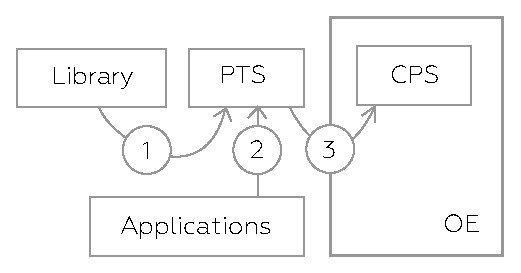
\includegraphics[scale=0.6]{minimal.eps}}
  \caption{Мінімальна система з чистої мови та інтерпретатора}
\end{figure}

\subsection{Максимальна система}
Інший приклад системи --- це максимальна система, яка містить усі формальні
мови програмування та формальне середовище виконання (порядок синтаксичних дерев
як параметрів при конструюванні мовної категорії може змінюватися, тут
генеалогія HTS не ведеться від MLTT, яке є розгалуженням).
\begin{equation}
Total = 
\begin{cases}
Ob: \{ O_{CPS}, O_{PTS}, O_{MLTT}, O_{ITS}, O_{HTS} \} \\
Hom: \begin{cases}
1,2: \mathbb{1} \rightarrow O_{HTS}, 3: O_{MLTT} \rightarrow O_{ITS} \\
4: O_{HTS} \rightarrow O_{ITS}, 5: O_{ITS} \rightarrow O_{PTS}, 6: O_{PTS} \rightarrow O_{CPS}
\end{cases}
\end{cases}
\end{equation}
За допомогою мереж Петрі це можна відобразити наступним чином:
\begin{figure}[ht]
  \centerline{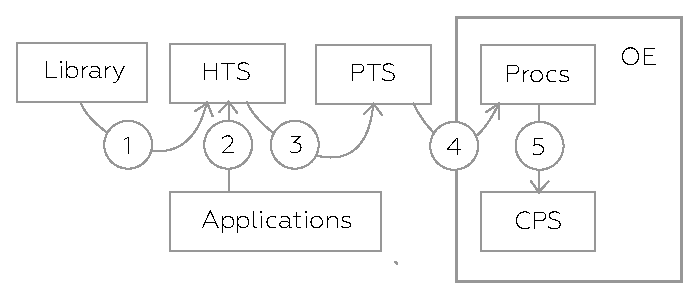
\includegraphics[scale=0.6]{higher.eps}}
  \caption{Кубічна та чиста системи типів та середовище виконання}
\end{figure}

\section{Формальні мови програмування}
Тут йдеться про мови програмування придатні для доведення теорем,
та їх таксономію від найелементарніших (чистої системи з одним типом $\Pi$) до
найпотужніших гомотопічних систем. Одна така гомотопічна система є кінцевим завданням
цього розділу --- побудова моделі гомотопічного верифікатора.
В процесі його побудови в цьому розділі ми розглянемо під
мікроскопом складові частини його нижчих мовних рівнів.

Застосуємо категорну семантику для мов програмування і будемо розглядати
мови програмування як моноїдальні мовні категорі, об'єкти яких є просторами
усіх програм цих мов програмування, а морфізми --- правила верифікації та компіляції цих мов.
Морфізми між мовними категоріями в категорї мов програмування --- це
функтори підвищення та пониження складності мови, подібно до того як діють
морфізми в контекстуальних категоріях. Морфізм деконструює або конструює за
допомогою Either-типу або $\Sigma$-типу індуктивний тип мови програмування.

Мови розкладаються у спектральну (індексовану натуральними числами $N \rightarrow U$)
послідовність мов, кожен елемент якої є мовою програмування,
яка не містить синтаксичне дерево вищої мови програмування.

\subsection{Чиста система типів $O_{PTS}$}

Чиста ситема або числення конструкцій або система з одим типом або
система з однією аксіомою, продовжує традиції елементарних пруверів
в стилі першого AUTOMATH та сучасних Henk, Morte, Cedile, Om.

\begin{definition} (Мовна категорія чистої мови $O_{PTS}$).
\begin{equation}
O_{PTS} =
\begin{cases}
Ob: \{\ X: maybe\ PTS, target: maybe\ CPS \ \} \\
Hom: \begin{cases}
type,norm: X \rightarrow X, extract: X \rightarrow target \\
certify: X \rightarrow target = type \circ norm \circ extract
\end{cases}
\end{cases}
\end{equation}
\end{definition}

\begin{definition} (Синтаксис мовної категорії $O_{PTS}$).
Чиста мова $O_{PTS}$ містить лише синтаксис одного типу, $\Pi$-типу.
Така теорія називається теорією з одним типом, або з однією аксіомою.
\begin{lstlisting}
data PTS = ppure (_: pts PTS)
\end{lstlisting}
\end{definition}

Вона описана в літературі як Calculus of Construction (Кокан),
Pure Type System (Стемп, Фу).

\begin{definition} (Синтаксичне дерево $O_\Pi$).
\begin{lstlisting}[mathescape=true]
data pts (lang: U)
   = star (n: nat)
   | var (x: name) (l: nat)
   | pi (x: name) (l: nat) (f: lang)
   | lambda  (x: name) (l: nat) (f: lang)
   | app (f a: lang)
\end{lstlisting}
\end{definition}

\subsection{Теорія типів Мартіна-Льофа $O_{MLTT}$}

Мова теорії типів є сучасною основою всіх пруверів з залежними типами,
такими, наприклад, як NuPRL та Agda. Багато так званих $\Pi\Sigma$ пруверів
імплементують $MLTT$ серед таких як:
$\Pi\Sigma$\footnote{\url{https://github.com/zlizta/pisigma-0-2-2}},
$\Pi\forall$\footnote{\url{https://github.com/sweirich/pi-forall}}.

\begin{definition} (Мовна категорія $O_{MLTT}$).
\begin{equation}
O_{MLTT} =
\begin{cases}
Ob: \{\ maybe\ MLTT\ \} \\
Hom: \begin{cases}
type,norm: Ob \rightarrow Ob \\
certify: Ob \rightarrow Ob = type \circ norm
\end{cases}
\end{cases}
\end{equation}
\end{definition}

\begin{definition} (Синтаксис мовної категорії $O_{MLTT}$).
Мова $O_{MLTT}$ включає в себе синтаксиси трьох типів
теорії Мартіна-Льофа: $O_\Pi$, $O_\Sigma$, $O_=$.
\begin{lstlisting}
data MLTT = mpure (_: pts MLTT)
          | msigma (_: exists MLTT)
          | mid (_: identity MLTT)
\end{lstlisting}
\end{definition}

\begin{definition} (Синтаксичне дерево $O_\Sigma$).
Також можна до чистої системи додати $\Sigma$-тип,
піднявши типову систему до мови $O_{MLTT-72}$ або $O_{\Pi\Sigma}$ :
\begin{lstlisting}[mathescape=true]
data exists (lang: U)
   = sigma (n: name) (a b: lang)
   | pair (a b: lang)
   | fst (p: lang)
   | snd (p: lang)
\end{lstlisting}
\end{definition}

\begin{definition} (Синтаксичне дерево $O_=$).
Додавши тип рівності можно підняти систему ще на одну сходинку,
до $O_{MLTT-84}$ або $O_{\Pi\Sigma=}$:
\begin{lstlisting}[mathescape=true]
data identity (lang: U)
   = id (t a b: lang)
   | id_intro (a b: lang)
   | id_elim (a b c d e: lang)
\end{lstlisting}
\end{definition}

\subsection{Система індуктивних типів $O_{ITS}$}

\begin{definition} (Мовна категорія $O_{ITS}$).
\begin{equation}
O_{ITS} =
\begin{cases}
Ob: \{\ X: maybe\ ITS, target: maybe\ CPS\ \} \\
Hom: \begin{cases}
type,norm,induction: X \rightarrow X, extract: X \rightarrow target \\
certify : X \rightarrow target \\
cerfity = type \circ norm \circ induction \circ extract \\
\end{cases}
\end{cases}
\end{equation}
\end{definition}

Мова індуктивних типів дозволяє безпосередньо кодувати індуктивні типи,
не використовуючи схеми кодування Бома, містить усі попередні мовні синтаксиси:
$O_=$, $O_\Sigma$, $O_\Pi$.

\begin{definition} (Синтаксичне дерево мовної категорії $O_{ITS}$).
\begin{lstlisting}
data ITS = ipure (_: pts ITS)
         | isigma (_: exists ITS)
         | iid (_: identity ITS)
         | iITS (_: ind ITS)
\end{lstlisting}
\end{definition}

Мова містить наступні допоміжні визначення: i) телескопу,
який містить послідовність елементів мови; ii) розгалуження,
як конструкцій case оператора; iii) імен конструкторів індуктивного типу.

\begin{lstlisting}
data tele   (A: U) = emp | tel (n: name) (b: A) (t: tele A)
data branch (A: U) =        br (n: name) (args: list name) (term: A)
data label  (A: U) =       lab (n: name) (t: tele A)
                         | com (n: name) (t: tele A) (dim: list name)
                               (s: list  (prod (prod name bool) A))
\end{lstlisting}

\begin{definition} (Синтаксичне дерево $O_*$).
Правило формації, конструктора та елімінатора визначається синтаксичним деревом $O_*$:
\begin{lstlisting}
data ind (lang: U)
   = datum  (n: name) (t: tele lang) (labels:   list (label lang))
   | case   (n: name) (t: lang)      (branches: list (branch lang))
   | ctor   (n: name)                (args:     list lang)
\end{lstlisting}
\end{definition}

\subsection{Гомотопічна система типів $O_{HTS}$}

\begin{definition} (Мовна категорія $O_{HTS}$).
$$
O_{HTS} =
\begin{cases}
Ob: \{\ maybe\ HTS\ \} \\
Hom: \begin{cases}
type,norm: Ob \rightarrow Ob \\
certify: Ob \rightarrow Ob = type \circ norm \\
\end{cases}
\end{cases}
$$
\end{definition}

\begin{definition} (Синтаксис мовної категорії $O_{HTS}$).
Синтаксис гомотопічної мовної категорії містить усі
попередні мовні синтаксиси: $O_I$, $O_W$, $O_=$, $O_\Sigma$, $O_\Pi$:
\begin{lstlisting}
data HTS = hpure (_: pts HTS)
         | hsigma (_: exists HTS)
         | hid (_: identity HTS)
         | hind (_: ind HTS)
         | homotopy (_: hts HTS)
\end{lstlisting}
\end{definition}

Гомотопічна типа наслідує $O_{ITS}$ але модифіковану з
Path-типом в індуктивних визначеннях, структурою композиції,
анонсує Path-тип (формація, конструктор, та елімінатор)
як лямбда функцію на відрізку, а також склейку типів у всесвіті
та склейку змінних з відповідними елімінаторами.

\begin{definition} (Синтаксичне дерево $O_I$).
\begin{lstlisting}
data hts (lang: U)
   = path (t a b: lang)
   | plam (n: name) (a: alg) (b: lang)
   | papp (f: name) (a: lang) (p: alg)
   | comp_ (a b: lang)
   | fill_ (a b c: lang)
   | glue_ (a b c: lang)
   | glue_elem (a b: lang)
   | unglue_elem (a b: lang)
\end{lstlisting}
\end{definition}

Таким чином,
$O_{HTS}$ містить два Id-типа, один унаслідований від $O_=$,
а інший який міститься в синтаксичному дереві $O_I$.

\section{Висновки}